\documentclass{llncs}

\usepackage[T1]{fontenc}
\usepackage{inconsolata}
\usepackage[polish]{babel}
\usepackage[utf8]{inputenc}
\usepackage{listings}
\usepackage{color}
\usepackage{enumerate}

\definecolor{pblue}{rgb}{0.13,0.13,1}
\definecolor{pgreen}{rgb}{0,0.5,0}
\definecolor{pred}{rgb}{0.9,0,0}
\definecolor{pgrey}{rgb}{0.46,0.45,0.48}

\usepackage{graphicx}
\usepackage{listings}
\lstset{language=Java,
  showspaces=false,
  showtabs=false,
  breaklines=true,
  showstringspaces=false,
  breakatwhitespace=true,
  commentstyle=\color{pgreen},
  keywordstyle=\color{pblue},
  stringstyle=\color{pred},
  basicstyle=\ttfamily\small,
}

\lstset{
  literate={ą}{{\k{a}}}1
           {ć}{{\'c}}1
           {ę}{{\k{e}}}1
           {ó}{{\'o}}1
           {ń}{{\'n}}1
           {ł}{{\l{}}}1
           {ś}{{\'s}}1
           {ź}{{\'z}}1
           {ż}{{\.z}}1
           {Ą}{{\k{A}}}1
           {Ć}{{\'C}}1
           {Ę}{{\k{E}}}1
           {Ó}{{\'O}}1
           {Ń}{{\'N}}1
           {Ł}{{\L{}}}1
           {Ś}{{\'S}}1
           {Ź}{{\'Z}}1
           {Ż}{{\.Z}}1
}


\begin{document}


\title{Opracowanie i implementacja podstaw optymalnego przechowywania i transferowania danych medycznych (ontologie)}

\author{Patryk Bąk, Marek Kendziorek, Wojciech Inglot}

\institute{AGH Kraków, 2013}
\maketitle


\section{Abstrakt}
\label{sec:Abstrakt}

Systemy medyczne należą do jednych z najbardziej rozbudowanych systemów w branży IT. Cechują się one nie tylko ogromnymi ilosciami danych, które przetwarzają, ale również bardzo dużą złożonoscią budowych tych danych oraz relacji, które między nimi zachodzą. Własnie branża e-health jako jedna z pierwszych zainteresowała się zastosowaniem ontologii oraz ich reprezentacji w zagadnieniu reprezentowania danych. Niniejszy artykuł porusza problem zastosowania optymalnych technologii i metodologii do implementacji systemu opartego o ontologię z naciskiem na przechowywanie oraz transfer ontologii.

Zaproponowane przez nas rozwiązanie problemu oparte zostało na języku programowania java oraz opartych na nim technologiach i narzędziach. Do transferu danych wykorzystano FUSEKI, które oferuje transfer danych protokołem REST z wykorzystaniem języka zapytań SPARQL. Dodatkowo przy definiowanu ontologii zaproponowano wykorzystanie opartego i interfejsy i stałe słownika danych.

Zaproponowana przez nas implementacja reprezentacji oraz transferu danych medycznych posiada wiele cech pożądanych przy projektowaniu tego typu systemów. Rozwiązanie to cechuje się bardzo dużą skalowalnoscią zarówno od strony wielkosci samego systemu jak i możliwosci rozbudowy przechowywanych w nim danych. Zastosowanie architektury typu SOA przy budowie systemu medyczneo pozwala na łatwą, modułową rozbudowę takiego systemu oraz ułatwioną integrację z innymi systemami medycznymi, zupełnie niezależnymi od siebie.



\begin{multicols}{2}

\section{Wstep}
\label{cha:wstep}

\subsection{Ontologia}
\label{sec:ont}

\subsection{OWL}
\label{sec:owl}

OWL (Ontology Web Language) jest opartym na składni XML językiem służącym do opisu ontologii. Stanowi on rozszerzenie języka RDF (Resource Definition Language). Istnieją 3 odmiany OWL: OWL Lite, OWL DL oraz OWL Full. W 2004 roku język ten został uznany za standard przez organizację W3C.

OWL został stworzony do przetwarzania informacji o obiektach oraz relacji między nimi, nie do przechowywania tych informacji w formie czytelnej dla człowieka. OWL jest zbudowany na bazie RDF, tak więc języki te są ze sobą w pełni kompatybilne. OWL posiada jednak znacznie mocniejszą składnię.

Do elementów języka OWL należą takie atrybuty jak:

\begin{itemize}

\item Class - definiuje grupę indywidualnosci, które posiadają pewne wspólne cechy. Klasy można organizować w hierarchie za pomocą atrybutu subClassOf.


\item rdf:Property - okresla pewne relacje między indywidualnosciami np. samochod może posiadać drzwi, osoba moze posiadać dziecko albo rodzica.

\item rdfs:domain - ogranicza indywidualności, do których można zastosować relację (property). Jeżeli relacja łączy jedną indywidualność z drugą, i jednocześnie posiada ona domenę na określoną klasę, to obie indywidualności muszą należeć do tej klasy.

\item rdfs:range - ogranicza nie tylko indywidualności, ale także wartość relacji (property)

\item Individual - indywidualności są instancjami klas, które są połączone pewnymi relacjami (property).

\end{itemize}

Wszystkie powyższe atrybuty są częścią specyfikacji OWL Lite.



\subsection{SPARQL}
\label{sec:sparql}

\subsection{REST}
\label{sec:rest}

REST jest protokołem komunikacji między aplikacjami, który tak naprawdę jest tylko pewną dodatkową warstwą nałożoną na protokół HTTP. Budowanie zapytań restowych z poziomu języków programowania jest tak samo proste, jak zrozumienie działania protokołu HTTP. Istnieje wiele bibliotek i prostych frameworków do budowania serwisów, odbierających i wysyłających zapytania HTTP. Należą do nich np Jersey-RS, czy zbudowana na jego bazie trochę większa biblioteka Apache CXF. Biblioteka Fuserki, będąca częścią specyfikacji Apache Jena oferuje możliwość transferu danych właśnie protokołem REST, przy użyciu języka zapytań SPAQRL. 

Ze względu na swoją prostotę i oparcie o standard HTT, wybór tego protokołu jako sposobu komunikacji między aplikacjami jest bardzo dobrą decyzją. Umożliwia to znakomitą skalowalność naszego systemu, poprzez rozdzielenie go na szereg indywidualnych aplikacji, które nie muszą być napisane przy użyciu tej samej technologii, muszą jedynie współdzielić tą metodę komunikacji oraz ewentualnie sposób serializacji danych.


\section{Implementacja rozwiązania}
\label{cha:impl}

Rozwiązanie zaprezentowane w niniejszym artykule zostało napisane w języku Java, z wykorzystaniem Ontology API biblioteki Apache Jena. Biblioteka ta pozwala na mapowanie różnego rodzaju reprezentacji ontologii na klasy Java. Do transferowania naszych danych wykorzystamy bibliotekę Apache CXF, a dokładniej jej moduł REST, który pozwoli nam na przesyłanie zserializowanych danych przez protokół HTTP.

\subsection{Reprezentacja danych}
\label{sec:persist}

Ontology API biblioteki Apache Jena pozwala między innymi na budowanie oraz importowanie modeli ontologii. Stworzenie nowego modelu ontologii oraz zaimportowanie do niego już istniejącej ontologii zapisanej w formacie OWL przedstawiono na rysunku.

\end{multicols}
\newpage
\begin{figure}[p]
	\centering
	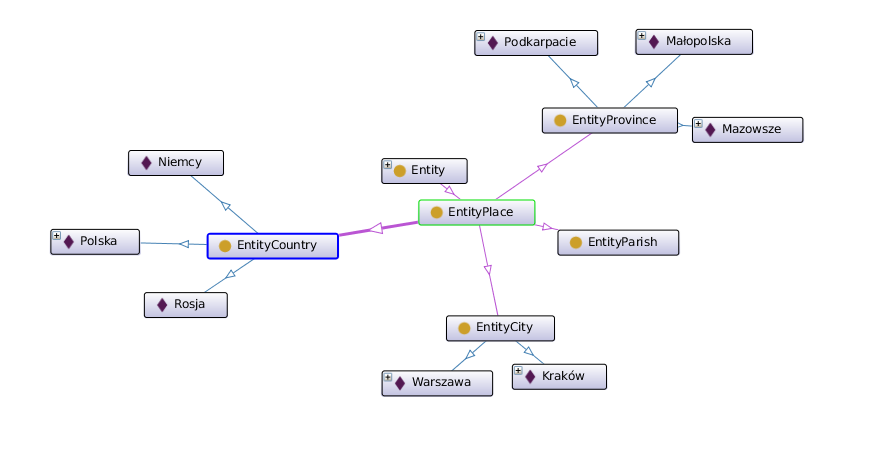
\includegraphics[scale=0.7, angle=90]{pics/EntityPlaceOntology}
	\caption{Przykład Ontologii Opartej o HL7 (EntityPlace)}
	\label{fig:placeont}
\end{figure}
\begin{figure}[p]
	\centering
	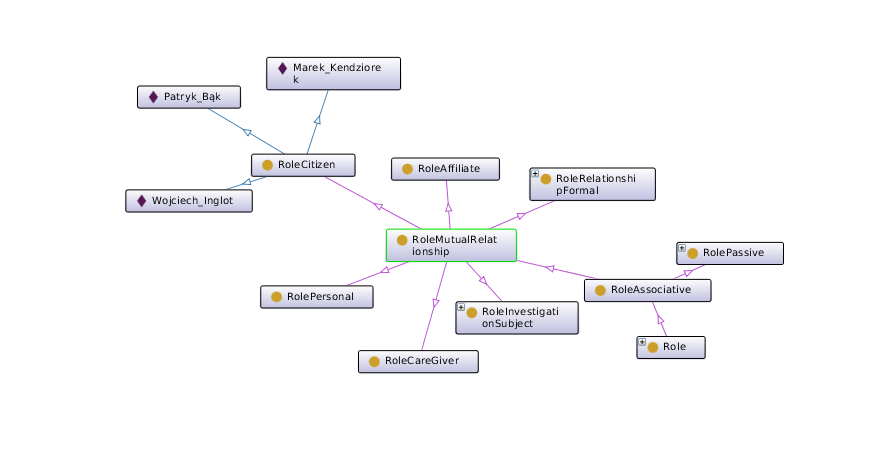
\includegraphics[scale=0.7, angle=90]{pics/RoleOntology}
	\caption{Przykład Ontologii Opartej o HL7 (Role)}
	\label{fig:placeont}
\end{figure}
\newpage
\begin{multicols}{2}

\subsection{Transfer danych}
\label{sec:transfer}

W projekcie uruchomiony został serwer HTTP Fuseki. Pozwala on na przechowywanie i udostepnienie danych wczytanych z plikow OWL poprzez zapytania HTTP. W jego wewnętrznej bazie danych budowane są grafu do których aplikacje klienckie odwołują się w zapytania SPARQL.

\subsubsection{Instalacja}

~Instalacja Jeny i Fuseki ogranicza się do dodania do zmiennych środowiskowych ścieżek do paczek.
\begin{lstlisting}
export JENA= /Users/XXXX/Fuseki/apache-jena-2.11.0/
export FUSEKI= /Users/XXXX/Fuseki/jena-fuseki-1.0.0/
\end{lstlisting}

\subsubsection{Uruchomienie serwera}

~Standardowo serwer FUSEKI uruchamiany jest pod wirtualną domeną \quotedblbase localhost\textquotedblright i na porcie 3030.

Uruchomienie serwera FUSEKI:
\begin{lstlisting}
./fuseki-server --update --loc=/Users/~/MyTDB/ /ds &
\end{lstlisting}

\subsubsection{Załadowanie pliku z ontologią}

~Załadowania pliku OWL (poprzez konsolową komendę):

\begin{lstlisting}
./s-put http://localhost:3030/ds/data default /Users/XXXX/RIMV3OWL.owl
\end{lstlisting}

\subsubsection{Tworzenie zapytania SPARQL}

~Wysłanie zapytania SPARQL wypisującego \quotedblbase koncepty\textquotedblright z załadowanego grafu:

\begin{enumerate}
\item Tworzenie zapytania.
\begin{lstlisting}
select distinct ?Concept where {[] a ?Concept}
\end{lstlisting}
\item Tworzenie zapytania HTTP POST, gdzie:
\begin{itemize}
\item jako URI podajemy sufix prowadzący do punktu końcowego (eng. endpoint) i doklajemy końcówkę /query
\item w parametrze POST/GET \quotedblbase query\textquotedblright podajemy stworzone zapytanie 
\item opcjonalne parametry: output (np. \quotedblbase json\textquotedblright ), default-graph-uri
\end{itemize}
\item W efekcie otrzymujemy zapytanie (dla punktu końcowego \quotedblbase ds\textquotedblright :
\end{enumerate}

\begin{lstlisting}
http://localhost:3030/ds/sparql? query=select+distinct++%3FConcept +where+%7B%5B%5D+a+%3FConcept%7D &default-graph-uri= &output=json
\end{lstlisting}
\section{Podsumowanie}
\label{cha:podsumowanie}

Zaproponowana przez nas implementacja reprezentacji oraz transferu danych medycznych posiada wiele cech pożądanych przy projektowaniu tego typu systemów. Rozwiązanie to cechuje się bardzo dużą skalowalnoscią zarówno od strony wielkosci samego systemu jak i możliwosci rozbudowy przechowywanych w nim danych. Zastosowanie architektury typu SOA przy budowie systemu medyczneo pozwala na łatwą, modułową rozbudowę takiego systemu oraz ułatwioną integrację z innymi systemami medycznymi, zupełnie niezależnymi od siebie. Idąc dalej można skorzystać również z możliwosci oferowanych przez narzędzia jeszcze wyższych rzędów, takie jak szyny biznesowe, dzięki którym integracja mogłaby być jeszcze skuteczniejsza, nie naruszając jednoczesnie architektur oraz implementacji poszczególnych systemów.

W kwestii reprezentacji danych, wykorzystanie takiego frameworku jak Apache Jena pozwala na intuicyjne operowanie na dowolnej reprezentacji ontologii, ich rozbudowę w srodowisku programowania java, oraz ich graficzną reprezentację. Wykorzystanie tutaj w pracy srodowiska java jednoczesnie czyni znacznie prostszą integrację tego rozwiązania z opisanym wczesniej mechanizmem transferowania informacji, który również napisany jest w tym języku.


\end{multicols}

\section*{Acknowledgments}\label{sec:Acknowledgments}

Authors would like to thank YYYYY.

\begin{thebibliography}{1}

\bibitem{Einstein}
A. Einstein, On the movement of small particles suspended in stationary liquids required by the molecular-kinetic theory of heat, Annalen der Physik 17, pp. 549-560, 1905.

\end{thebibliography}

\end{document}